\section*{Problem 12 - Linear and decision-feedback MIMO detection}
\begin{align*}
	& \text{\uline{MIMO-MRC}} \\
	& \sigma_{n_1}^2=\sigma_{n_2}^2=\ldots=\sigma_{N_R}^2=\sigma_n^2 \\
	& 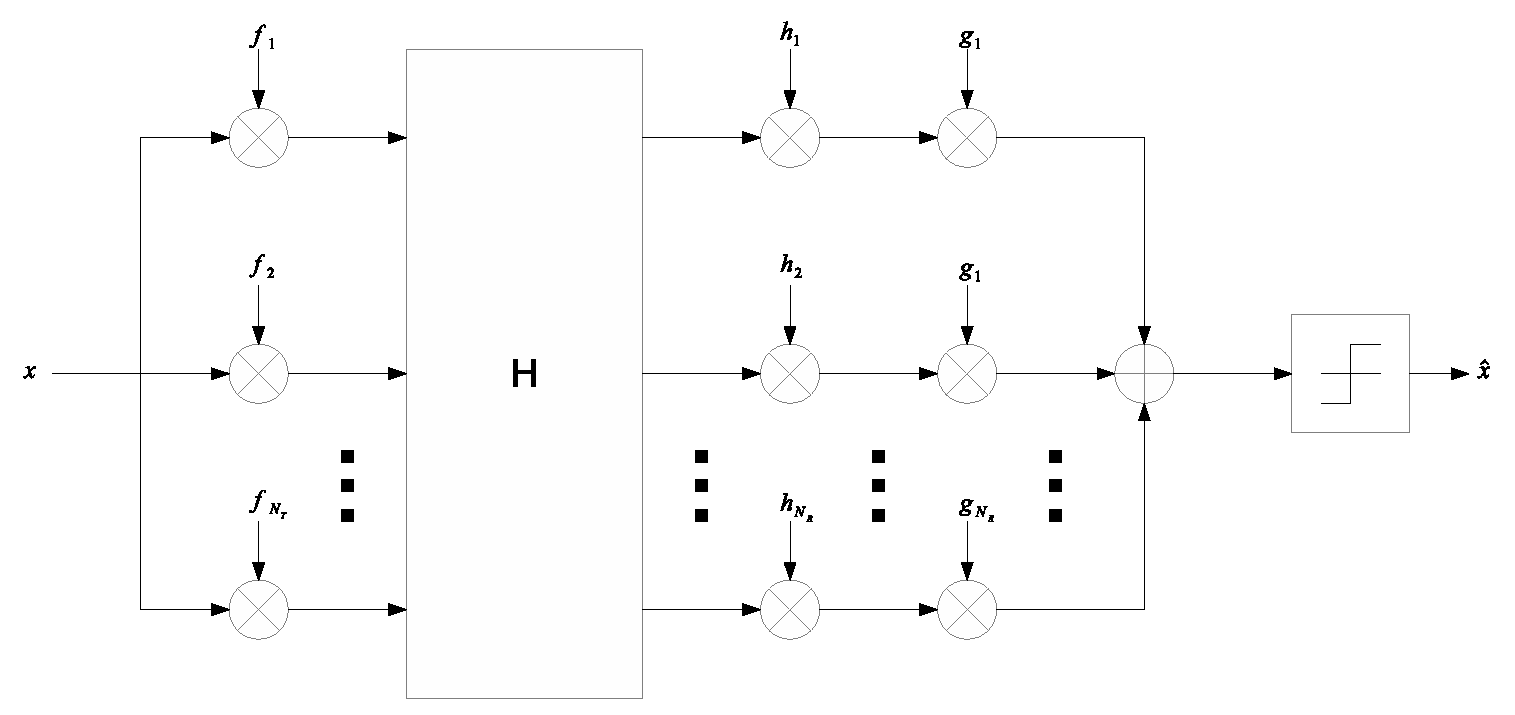
\includegraphics[width=1\textwidth]{MIMO_MRC.eps} \\
	& f=\left(f_1,f_2,\ldots,f_{N_R}\right)^T;\qquad g=\left(g_1^*,g_2^*,\ldots,g_{N_R}^*\right) \\
	& \quad\rightarrow\quad\text{Nomenclature:}\quad
	\begin{cases}
	f^Hf=1=\|f\|^2 \\
	g^Hg=1=\|g\|^2
	\end{cases} \\
	& \text{singular value decomposition:}\quad\mathbf{H=U\Sigma V}^H \\
	& \mathbf{\Sigma} =\diag\left(\xi_1^2,\xi_2^2,\ldots,\xi_N^2\right) \\
	& \quad\rightarrow\quad\text{sorted in descending order}\quad\rightarrow\quad\xi_1^2=\xi_{max}^2 \\
	& f = \mathbf{V}f'\quad\rightarrow\quad\mathbf{V}^Hf=\underbrace{\mathbf{V}^H\mathbf{V}}_{\mathbf{I}}f'=f'\quad\rightarrow\quad\|f'\|^2=\|\mathbf{V}^Hf\|^2\overset{\mathbf{V}: unitary}{=}\|f\|^2=1 \\
	& \text{in a similar way:} \\
	& \quad\rightarrow\quad g=u\cdot g' \\
	& \quad\rightarrow\quad \|g\|^2=\|g'\|^2=1 \\
	& \mathrm{SNR}=\frac{\sigma_x^2\left|\overbrace{h_{total}}^{\substack{\text{total transfer} \\ \text{function}}}\right|^2}{\sigma_n^2\underbrace{\|g\|^2}_{\rightarrow =1}}= \frac{\sigma_x^2\left|g^HHf\right|}{\sigma_n^2}=\frac{\sigma_x^2\left|g'^H\mathbf{U}^H\mathbf{U\Sigma V}^H\mathbf{V}f'\right|}{\sigma_n^2} \\
\end{align*}
\begin{align*}
	& \quad\rightarrow\quad\mathrm{SNR}=\frac{\sigma_x^2}{\sigma_n^2}\left|g'^H\mathbf{\Sigma}f'\right| \\
	& g'=\begin{pmatrix}1&0&\ldots&0\end{pmatrix}';\quad f'=\begin{pmatrix}1&0&\ldots&0\end{pmatrix}' \\
	& \quad\rightarrow\quad\text{to maximize SNR: }\xi_1=\xi_{max} \\
	& \quad\quad\quad\mathrm{SNR_{max}}=\frac{\sigma_x^2}{\sigma_n^2}\xi_1^2 \\
	& \text{$\xi_k^2$ are also eigenvalues of $HH^H$} \\
	& \quad\|H\|_F^2=\tr\left(HH^H\right)=\sum\limits_{k=1}^N\xi_k^2\qquad N=\min\{N_T,N_R\} \\
	& \text{Frobenius norm} \\
	& \xi_1^2=\xi_{max}^2\quad\rightarrow\quad\underbrace{\frac{1}{N}\sum\limits_{k=1}^N\xi_k^2}_{\text{average}}\le\xi_{max}^2\le\sum\limits_{k=1}^N\xi_k^2 \\
	& \|H\|_F^2=\sum\limits_{i=1}^{N_T}\sum\limits_{j=1}^{N_R}\left|h_{ij}\right|^2,\quad h_{ij}\sim C\mathcal{N}\left(0,1\right) \\
	& \quad\rightarrow\quad\|H\|_F^2\text{ is the sum of squared complex Gaussian RVs} \\
	& \quad\rightarrow\quad\text{$\chi^2$-square ($\chi^2$-distribution} \\
	& f_{{\|H\|}_F^2}\left(x\right)=\frac{1}{\Gamma\left(N_TN_R\right)}x^{N_TN_R-1}e^{-x} \\
	& \overbrace{f_{\frac{1}{N}{\|H\|}_F^2}}^{\text{pdf of the channel}}=\frac{1}{\Gamma\left(N_TN_R\right)}\left(Nx\right)^{N_TN_R-1}e^{-Nx} = \frac{N^{N_TN_R}x^{N_TN_R-1}e^{-Nx}}{\Gamma\left(N_TN_R\right)} \\
	& \overline{\mathrm{SER}}\ge\int\limits_0^\infty f_{\frac{1}{N}{\|H\|}_F^2}\mathrm{SER}\left(x\right)\mathrm{d}x = \int\limits_0^\infty\frac{N^{N_TN_R}x^{N_TN_R-1}e^{-Nx}}{\Gamma\left(N_TN_R\right)}\frac{C_\mathcal{A}}{2}e^{-\frac{d_\mathcal{A}^2}{2}x\gamma}\mathrm{d}x= \\
	& \qquad=\frac{N^{N_TN_R}C_\mathcal{A}}{2\Gamma\left(N_TN_R\right)}\int\limits_0^\infty x^{N_TN_R-1}e^{-\left(N+\frac{d_\mathcal{A}^2}{2}\gamma\right)x}\mathrm{d}x=\frac{N^{N_TN_R}C_\mathcal{A}}{2\Gamma\left(N_TN_R\right)}\frac{\Gamma\left(N_TN_R\right)}{\left(N+\frac{d_\mathcal{A}^2}{2}\gamma\right)^{N_TN_R}} \\
	& \rightarrow\quad\overline{\mathrm{SER}}\ge\frac{C_\mathcal{A}N^{N_TN_R}}{2\left(N+\frac{d_{\mathcal{A}^2}}{2}\underbrace{\gamma}_{\mathrm{SNR}}\right)^{N_TN_R}} \\
	& \mathrm{SNR}\quad\rightarrow\quad\infty\quad\Rightarrow\quad\mathrm{SER}\ge\frac{C_\mathcal{A}}{2\left(\frac{d_\mathcal{A}^2}{2N}\gamma\right)^{N_TN_R}}
\end{align*}
\begin{align*}
	& \frac{\sum\limits_{k=1}^N\xi_k^2}{N}\le\xi_{max}^2\le\sum\limits_{k=1}^N\xi_k^2\quad\rightarrow\quad\overline{\mathrm{SER}}\le\frac{C_\mathcal{A}}{2\left(\frac{D_\mathcal{A}^2}{2}\gamma\right)^{N_TN_R}} \\
	& \quad\rightarrow\quad\frac{C_\mathcal{A}}{2\left(\frac{D_\mathcal{A}^2}{2N}\gamma\right)^{N_TN_R}}\le\overline{\mathrm{SER}}\le\frac{C_\mathcal{A}}{2\left(\frac{D_\mathcal{A}^2}{2}\gamma\right)^{N_TN_R}} \\
	& \text{we have: }\frac{\ldots}{\ldots\gamma^{N_TN_R}}\quad\rightarrow\quad\text{Diversity gain $=N_TN_R$} \\
\end{align*}
\begin{align*}
	& \text{equalization}
	& \begin{cases}
		\substack{\text{at the receiver}\\ \text{(detection)}} 
			\begin{cases}
				\text{linear} 
					\begin{cases}
						\text{Zero-Forcing ZF} \\
						\text{Minimum Mean Square Error MMSE}
					\end{cases} \\
				\text{decision feedback}
					\begin{cases}
						\text{ZF} \\
						\text{MMSE}
					\end{cases}
			\end{cases} \\
		\substack{\text{at the transmitter}\\ \text{(precoding)}}
			\begin{cases}
				\text{linear} \\
				\text{with feedback}
			\end{cases}
	\end{cases} \\
	& \text{Linear equalizer:} \\
\end{align*}